\item Een hockeyschijf of puck krijgt op een bevroren vijver een horizontale slag waardoor het met een snelheid van $20,5~\rm m/s$ vertrekt. Na hoeveel meter komt de puck tot rust als de wrijvingsfactor tussen de puck en het ijs 0,18 bedraagt? %Na $120~\rm m$ komt de puck tot rust. Bepaal de wrijvingsfactor.
\begin{oplossing}
\begin{figure}[h]
\begin{center}
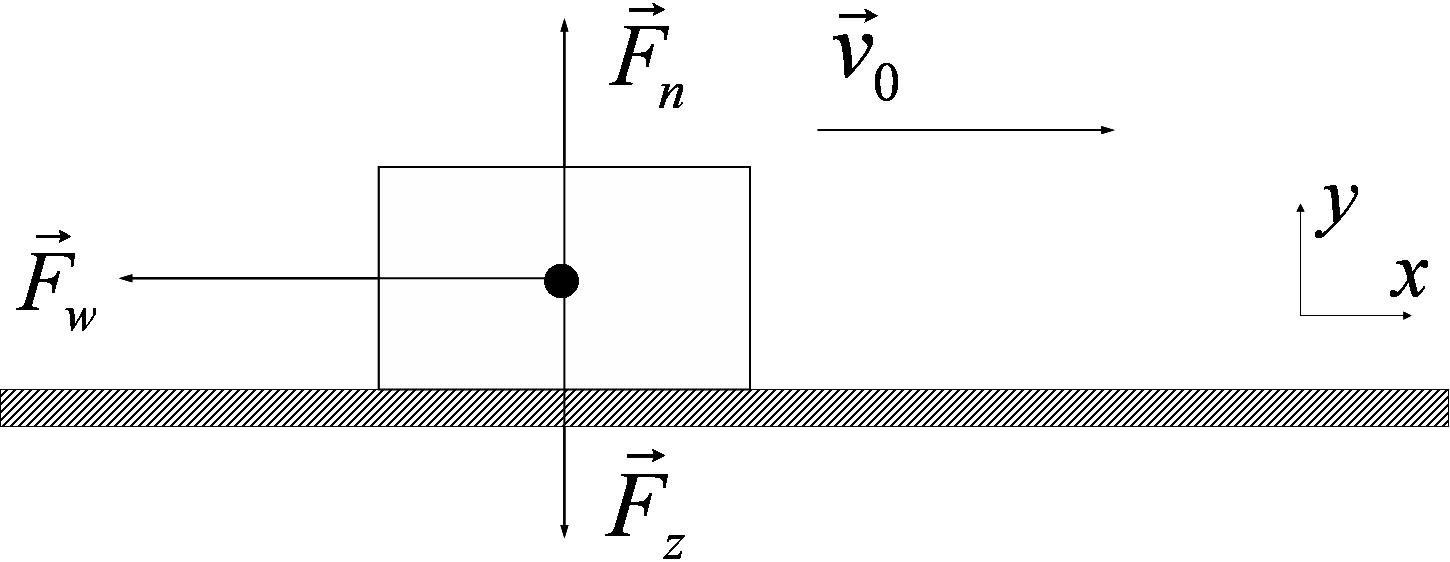
\includegraphics[width=0.5\textwidth ,angle=0]{hockeypuck2}
\end{center}
\end{figure}
\newline
\item [\textit{gegeven}]
\begin{tabular}[t]{lcl}
$v_0$ &$=$& $20,5~\rm m/s$\\
$x$ &$=$& $120~\rm m$\\
\end{tabular}
\item [\textit{gevraagd}]
$\mu$
\item [\textit{oplossing}]
De wrijvingskracht is de enige kracht volgens de horizontale
richting en vormt dus de resulterende kracht. Omdat ze tegengesteld
is aan de $x$-as geldt $F_{w,x}=-F_w$. Met $F_w=\mu F_n$ vinden we
voor de versnelling:
\begin{eqnarray}
-F_w &=& ma\nonumber\\
&\Downarrow& \nonumber\\
-\mu mg &=&ma\nonumber\\
&\Updownarrow& \nonumber\\
a &=& -\mu g\label{a}
\end{eqnarray}
De tijd uit de vergelijkingen voor een EVRB elimineren, waarbij de
eindsnelheid $v$ en de beginpositie $x_0$ nul zijn, levert:
\begin{eqnarray}
v&=&v_0+at\nonumber\\
x&=&x_0+v_0t+\frac{1}{2}at^2\nonumber\\
&\Downarrow&\nonumber\\
0&=&v_0+at\Leftrightarrow t=-\frac{v_0}{a}\nonumber\\
x&=&v_0\left(-\frac{v_0}{a}\right)+\frac{1}{2}a\left(-\frac{v_0}{a}\right)^2\nonumber\\
&\Downarrow&\nonumber\\
a&=&-\frac{v_0^2}{2x}\label{-v_0^2/2x}
\end{eqnarray}
Vergelijking (\ref{-v_0^2/2x}) samen met (\ref{a}) levert dan:
\begin{eqnarray}
\mu &=& \frac{v_0^2}{2gx}\label{remvgl}\\
&&\nonumber\\
&=& 0,178\nonumber
\end{eqnarray}
\end{oplossing}